\documentclass[journal]{IEEEtran}
%\usepackage{cite}
\usepackage{graphicx}
%\usepackage{circuitikz}
%\usepackage[cmex10]{amsmath}
%\usepackage{dblfloatfix}
%\usepackage{capt-of}
%\usepackage{breqn}
%\usepackage{listings}
%\usepackage{mathrsfs}
%\usepackage[scale=.8]{geometry}
%\usepackage{hyperref}
%\usepackage{breakurl}
\usepackage{epstopdf}
\usepackage[nomarkers,nolists,tablesfirst]{endfloat}
\renewcommand{\efloatseparator}{\mbox{}}

\begin{document}
% paper title
% can use linebreaks \\ within to get better formatting as desired
\title{A Switched-Capacitor Amplifier for Use in a 2.5bit/stage Pipelined Analog-to-Digital Converter }

\author{Joseph Meyer and Miles Sherman}

% The paper headers
\markboth{ELEN 6312 Advanced Analog Integrated Circuits}%
{Shell \MakeLowercase{\textit{et al.}}: Bare Demo of IEEEtran.cls for Journals}

\maketitle

\begin{abstract}
A switched-capacitor amplifier with a nominal gain of 4 was designed for use in a 2.5 bit/stage pipelined analog-to-digital converter (ADC). The total resolution of the ADC was 10 bits. The sample rate of the ADC was $5kS/s$. The amplifier consisted of 4 sample capacitors and 1 hold capacitor in feedback around an operational transconductance amplifier (OTA). The OTA consisted of a pMOS-input folded cascode stage followed by an nMOS common source stage. The open loop DC gain of the OTA was $110.9dB$. The unity gain bandwidth of the OTA was $87.1kHz$. The circuit consumed MAKE THIS MORE ACCURATE $725nW$ of DC power. SOMETHING ABOUT EFFECTIVE NUMBER OF BITS. SOMETHING ABOUT FIGURE OF MERIT.
\end{abstract}

% Note that keywords are not normally used for peerreview papers.
\begin{IEEEkeywords}
switched-capacitor amplifier, pipelined analog-to-digital converter
\end{IEEEkeywords}

\section{Introduction}
\IEEEPARstart {P}{ipelined} 2.5 bit/stage ADCs require accurate 

\section{System Level Design}
\subsection{Top Level Schematic}

\subsection{Sample and Hold Capacitors}

\subsection{Switches}

\section{Transistor Level OTA Design}
\subsection{Gain Stage}

\subsection{Biasing}

\subsection{Component Values}

\begin{table}
\centering
\caption{Passive Component Values}
\label{tab:passive_elements}
\begin{tabular}{|c|c|}
\hline Component & Value \\ 
\hline Resistors & $\Omega$ \\ 
\hline  &  \\ 
\hline Capacitors & $F$ \\ 
\hline  &  \\ 
\hline  &  \\ 
\hline  &  \\ 
\hline 
\end{tabular} 
\end{table}

\begin{table}
\centering
\caption{Transistor Sizings}
\label{tab:trans_sizes}
\begin{tabular}{|c|c|c|c|}
\hline Transistor & Width (m) & Length (m) & Aspect Ratio \\ 
\hline  &  &  &  \\ 
\hline  &  &  &  \\ 
\hline  &  &  &  \\ 
\hline  &  &  &  \\ 
\hline  &  &  &  \\ 
\hline  &  &  &  \\ 
\hline  &  &  &  \\ 
\hline 
\end{tabular} 
\end{table}




%%%%%%%%%%%%%%%%%%%%%%%%%%%%%%%
\section{Open Loop OTA Results}
Upon completion of our OTA design, we performed various open-loop simulations to verify that we had met our required specifications.

\subsection{Open Loop Differential Frequency Response}
Keeping the entire switch capacitor system in perspective, the most important specs for us to hit were those for differential gain for total accuracy and unity-gain bandwidth (UGB) for total speed. Therefore, we measured those performance values for our OTA first. As can be seen in our differential gain plot (Figure \ref{fig:open_dm_gain}), we successfully hit our specs for gain and UGB across all three PVT corners (see Table \ref{tab:specs_results}). The plot also shows that we were able to use compensation capacitance to push our dominant pole to a very low frequency ($\approx0.1 Hz$).

We also plotted the phase response of our open loop OTA (see Figure \ref{fig:open_dm_phase}). From this plot, the low frequency pole seen in the gain response is confirmed. In addition, it can clearly be seen that the additional poles and the zero created by the compensation capacitor has been pushed out beyond our unity-gain bandwidth. Our phase margin measurements are shown to be very consistent across PVT corners and all above our spec (see Figure \ref{tab:specs_results}).

\begin{figure}
\centering
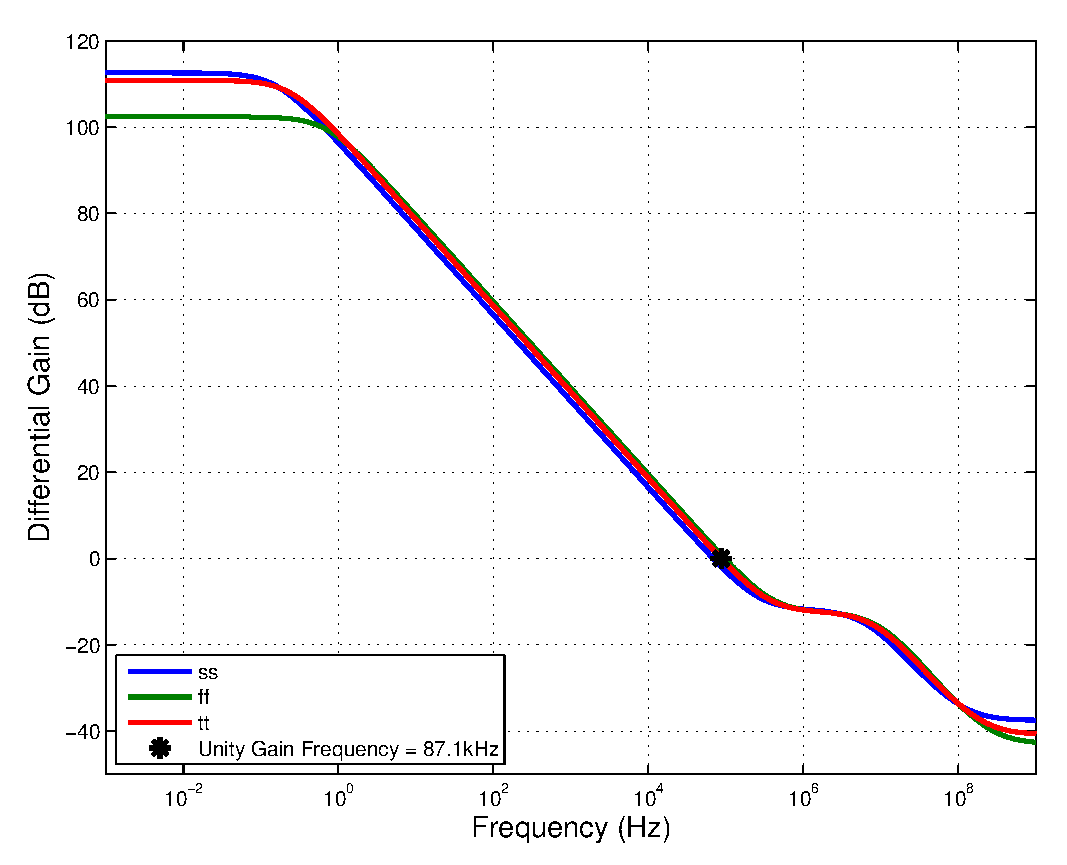
\includegraphics[width=4in]{Plots/open_dm_gain.eps}
\caption{The open loop differential gain magnitude response of the OTA.}
\label{fig:open_dm_gain}
\end{figure}


\begin{figure}
\centering
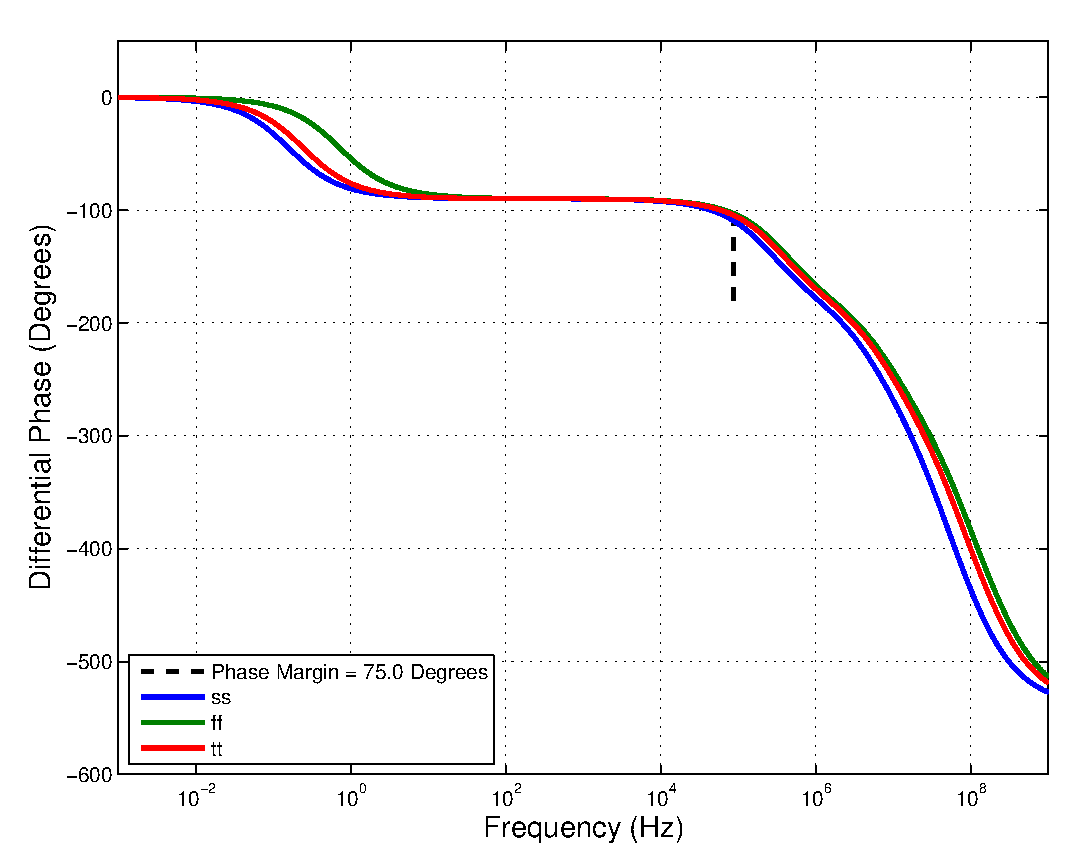
\includegraphics[width=4in]{Plots/open_dm_phase.eps}
\caption{The open loop differential gain phase response of the OTA.}
\label{fig:open_dm_phase}
\end{figure}

\subsection{Open Loop Common Frequency Mode Response}
In order for our OTA to be robust against common-mode noise, it is important for the common mode gain to remain very low across all frequencies. As can be seen in our plots for common mode gain (Figure \ref{fig:open_cm_gain}) and common mode phase (Figure \ref{fig:open_cm_phase}), common mode changes on the input have a very limited effect on the output.

\begin{figure}
\centering
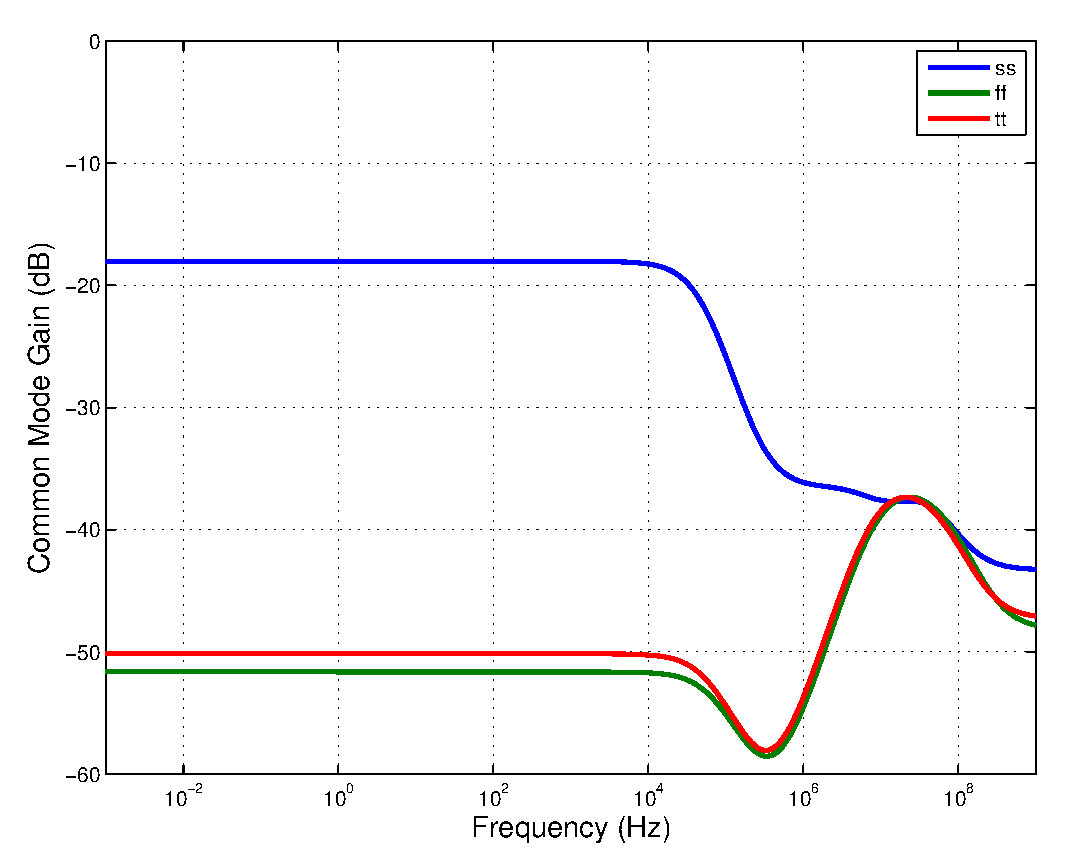
\includegraphics[width=4in]{Plots/open_cm_gain.eps}
\caption{The open loop common mode gain magnitude response of the OTA.}
\label{fig:open_cm_gain}
\end{figure}

\begin{figure}
\centering
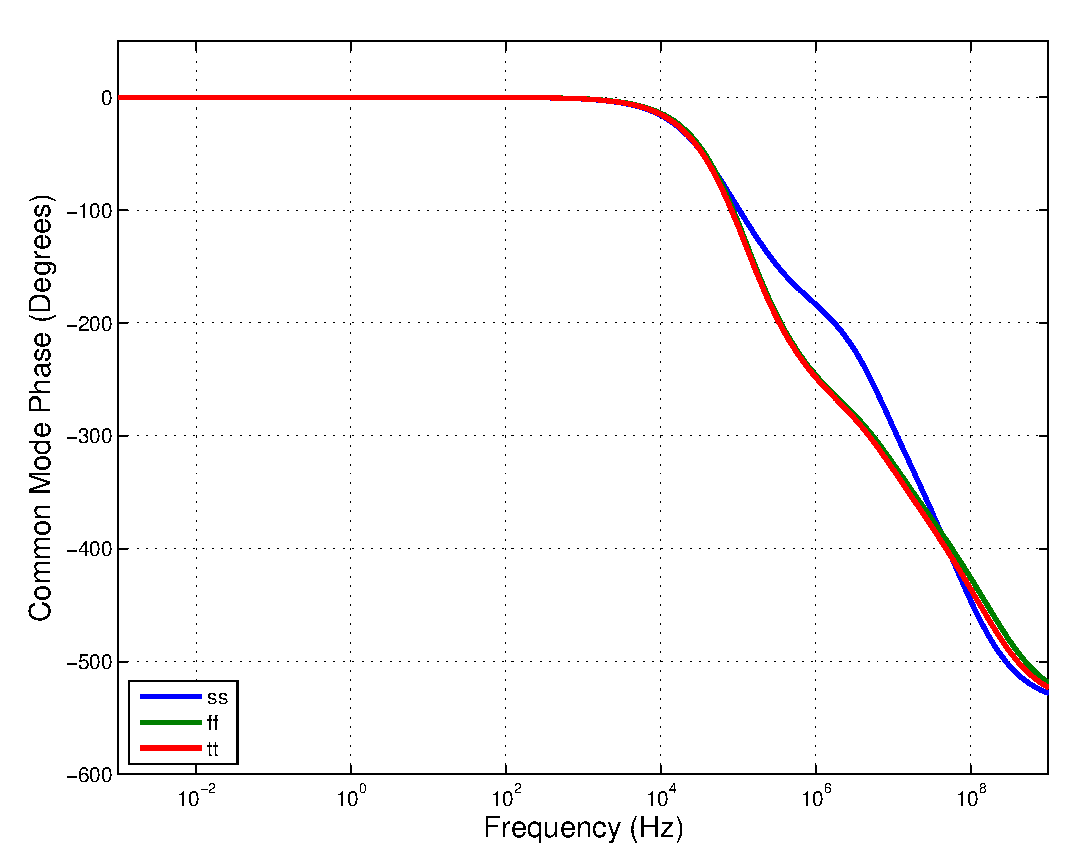
\includegraphics[width=4in]{Plots/open_cm_phase.eps}
\caption{The open loop common mode gain phase response of the OTA.}
\label{fig:open_cm_phase}
\end{figure}

\subsection{Common Mode Feedback Frequency Response}
Our goal in developing a common mode feedback (CMFB) network was to provide circuitry to hold our output node at $V_{CM}$. To ensure that our circuit was functioning as we intended, we broke our feedback loop at the input of the CMFB network and stimulated the circuit with a small signal source. We then measured the output of the CMFB circuit at the node that feeds back to our cascade branch. Our results can be seen in figures \ref{fig:open_cmfb_gain} and \ref{fig:open_cmfb_phase}.

\begin{figure}
\centering
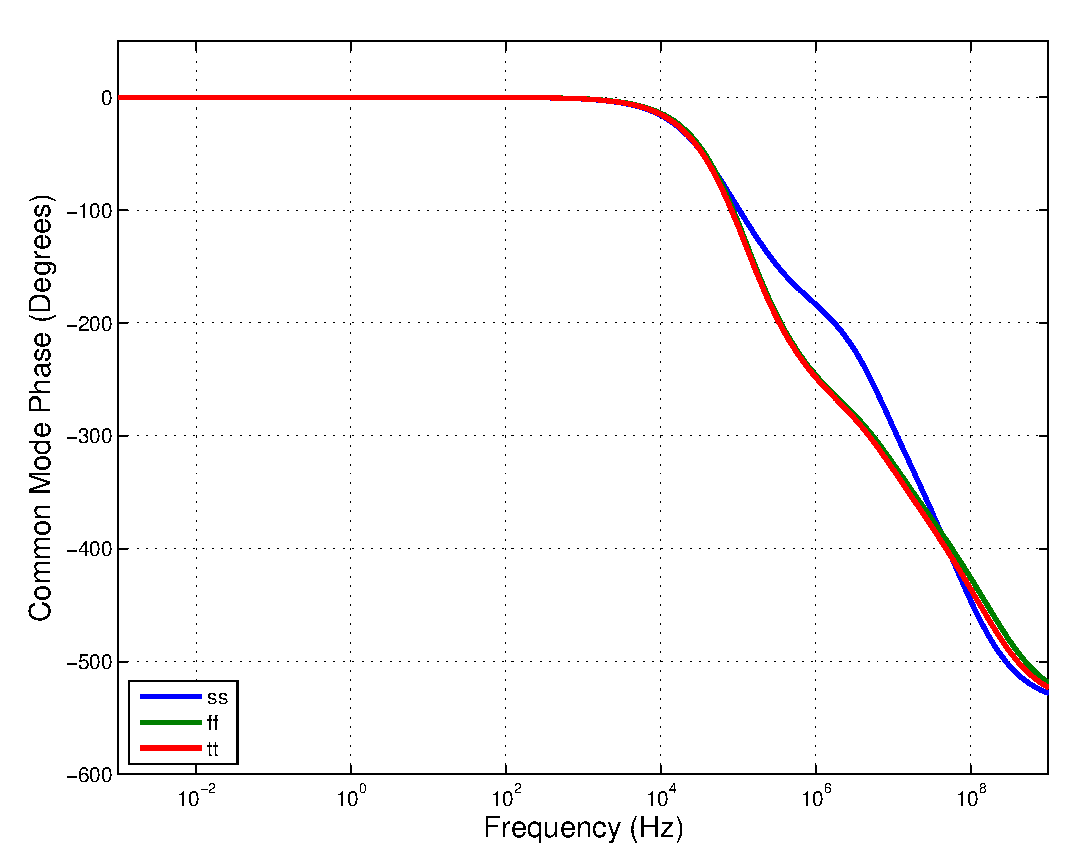
\includegraphics[width=4in]{Plots/open_cm_phase.eps}
\caption{The common mode feedback network gain phase response.}
\label{fig:open_cmfb_gain}
\end{figure}

\begin{figure}
\centering
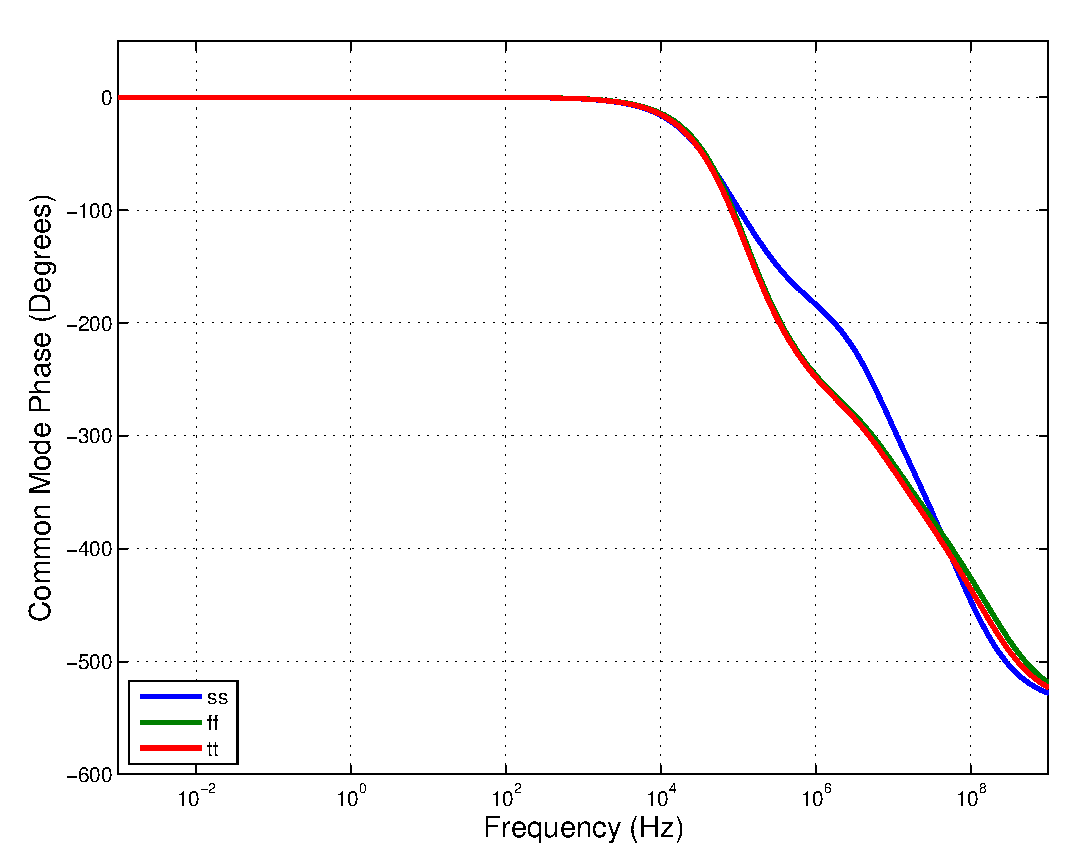
\includegraphics[width=4in]{Plots/open_cm_phase.eps}
\caption{The common mode feedback network gain magnitude response.}
\label{fig:open_cmfb_phase}
\end{figure}


\section{Closed Loop Amplifier Results}
After we verified that we had met our open loop OTA specifications, we replaced the ideal OTA in our system level design with our own OTA design to verify that we still met the system level specifications.

\subsection{Nyquist Rate Sinusoidal Transient Response}
The first test we ran on our system was a sine wave input at our full-scale amplitude and the Nyquist frequency. As can be seen in our plot (Figure \ref{fig:closed_sine}), our system samples the input at the end of the sample phase to be $0.35V$ ($V_{FS}$). Over the course of the hold phase, the output slews and then settles linearly to a value of $1.402V$. This is within our maximum error value (shown below) and shows that our circuit successfully handles a sine wave input. The maximum input referred error we can tolerate is

\begin{equation}
4*\frac{V_{LSB}}{2} = 5.4mV
\end{equation}

\begin{figure}
\centering
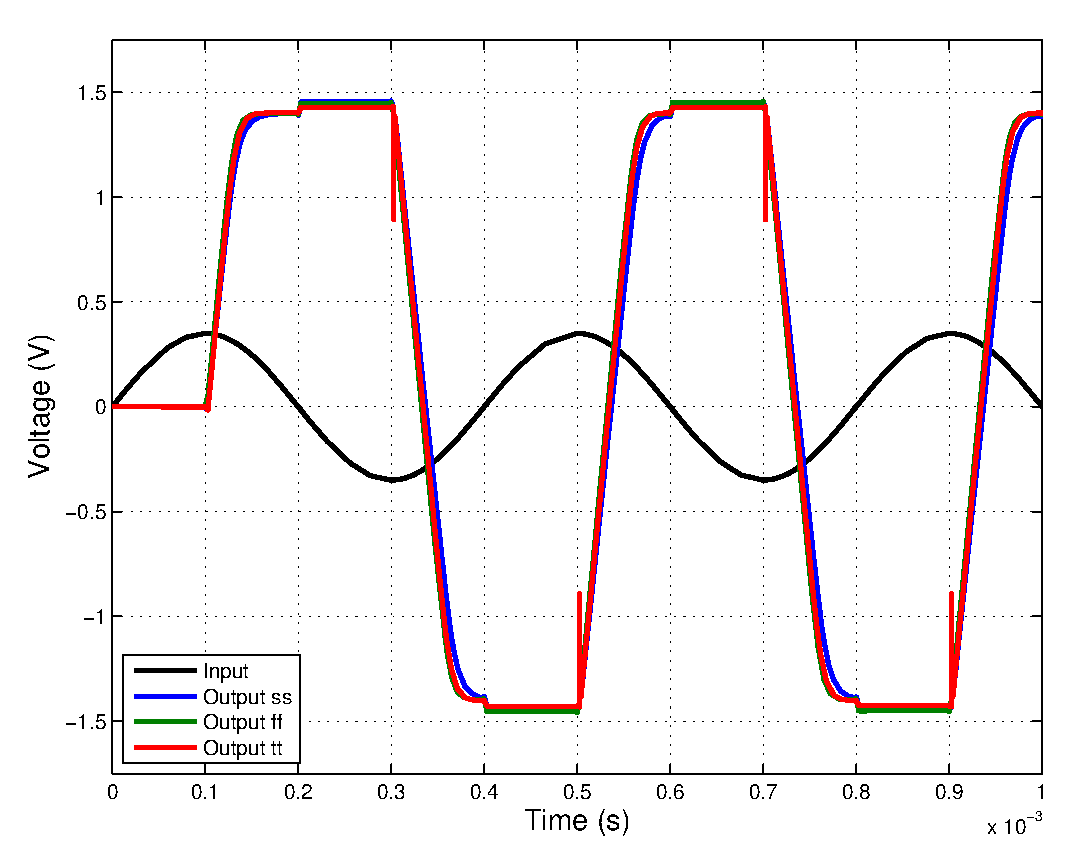
\includegraphics[width=4in]{Plots/closed_sine.eps}
\caption{The closed loop transient response to a full-scale amplitude sinusoid at the Nyquist frequency.}
\label{fig:closed_sine}
\end{figure}


\subsection{Small Step Transient Response}
The second test we performed on our closed loop system was a small step input. As can be seen in figure \ref{fig:closed_small_step}, our output shows a fast settling with little to no slewing. We provided an input step of $2mV$ and observed the output to settle to $8.012mV$ at the end of the hold phase. This is well within our spec for error so this test was successful.

\begin{figure}
\centering
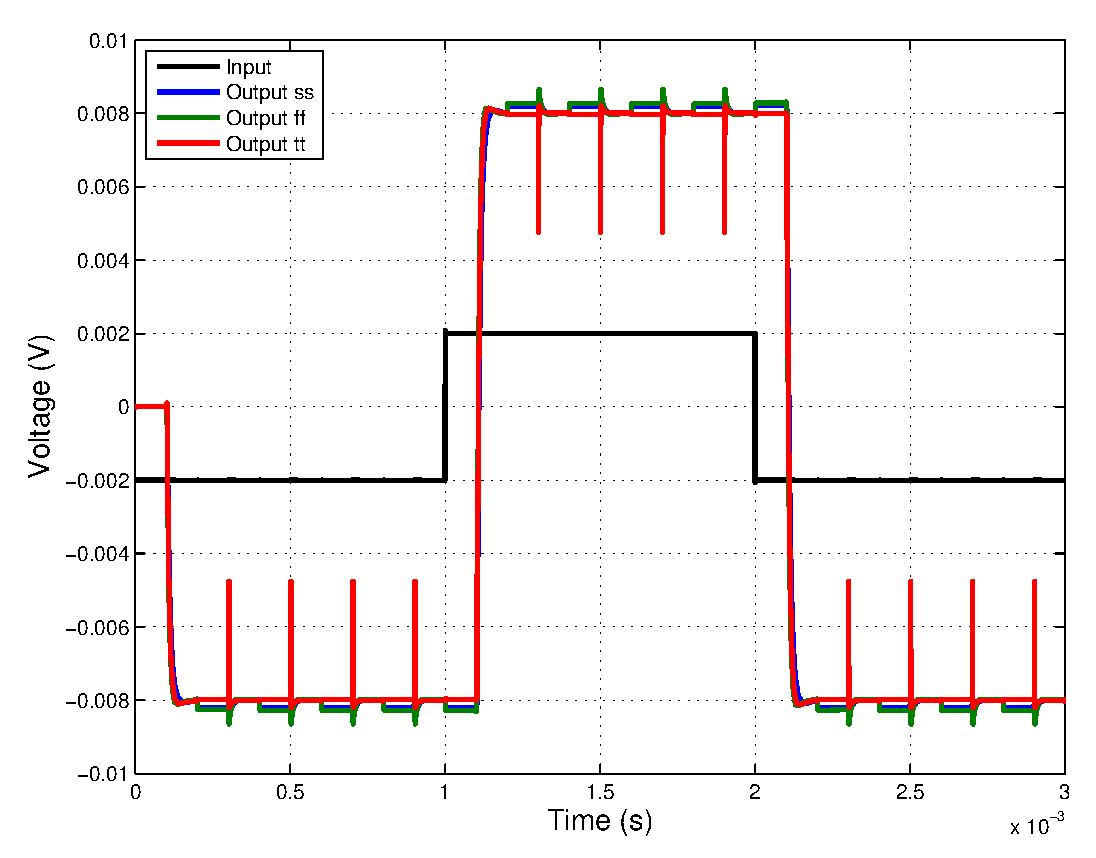
\includegraphics[width=4in]{Plots/closed_small_step.eps}
\caption{The closed loop transient response to a small amplitude step input.}
\label{fig:closed_small_step}
\end{figure}


\subsection{Full Scale Step Transient Response}
The third test we performed on our closed loop system was a step input at the full-scale voltage. The results of this test closely resembled those of the sine wave input. The reason for this is that the input is again sampled at the full-scale voltage and the output settles accordingly. This test was successful.

\begin{figure}
\centering
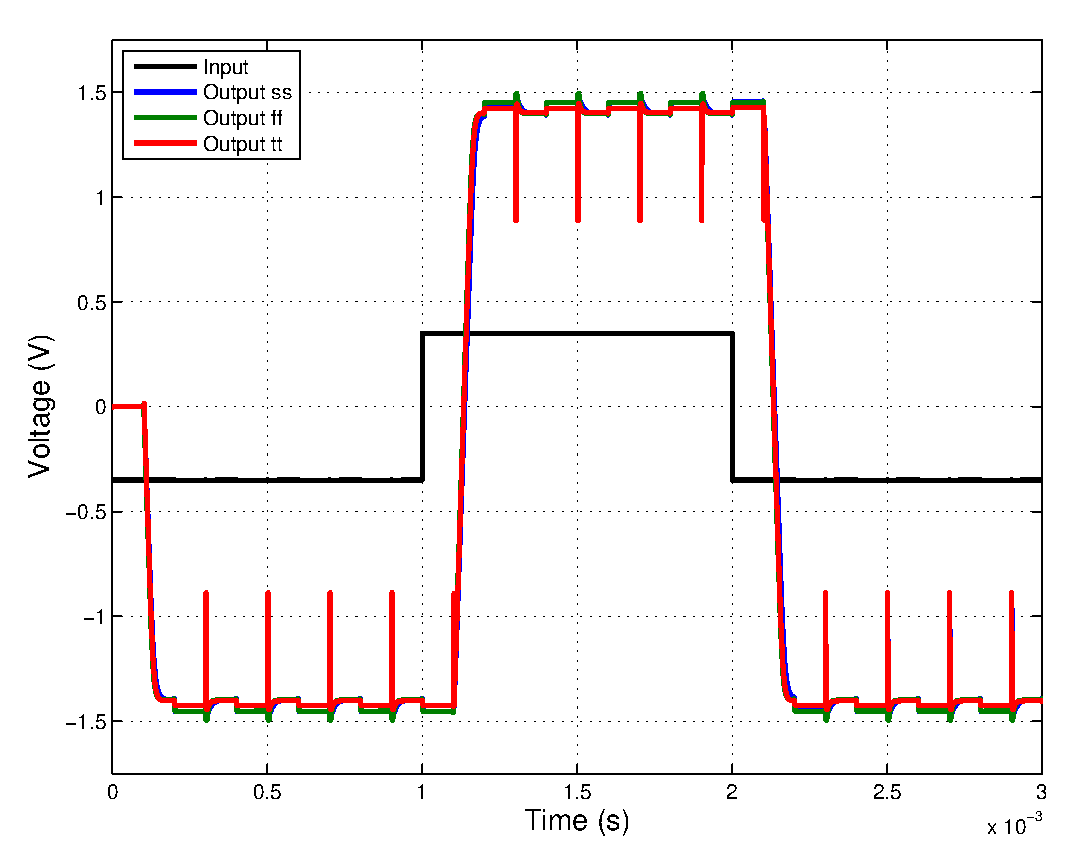
\includegraphics[width=4in]{Plots/closed_large_step.eps}
\caption{The closed loop transient response to a full-scale amplitude step input.}
\label{fig:closed_large_step}
\end{figure}

\subsection{Sawtooth Transient Response}
The fourth and final test we performed on our closed loop system was a sawtooth input at $f_s/20$. As can be seen from our plot in figure \ref{fig:closed_saw}, our system has no problem settling to the correct output for small changes in the input (along the ramp of the sawtooth). In addition, our output settles to the correct output in time after the edge of the sawtooth when the input drops from the full-scale voltage to the negative full-scale voltage.

\begin{figure}
\centering
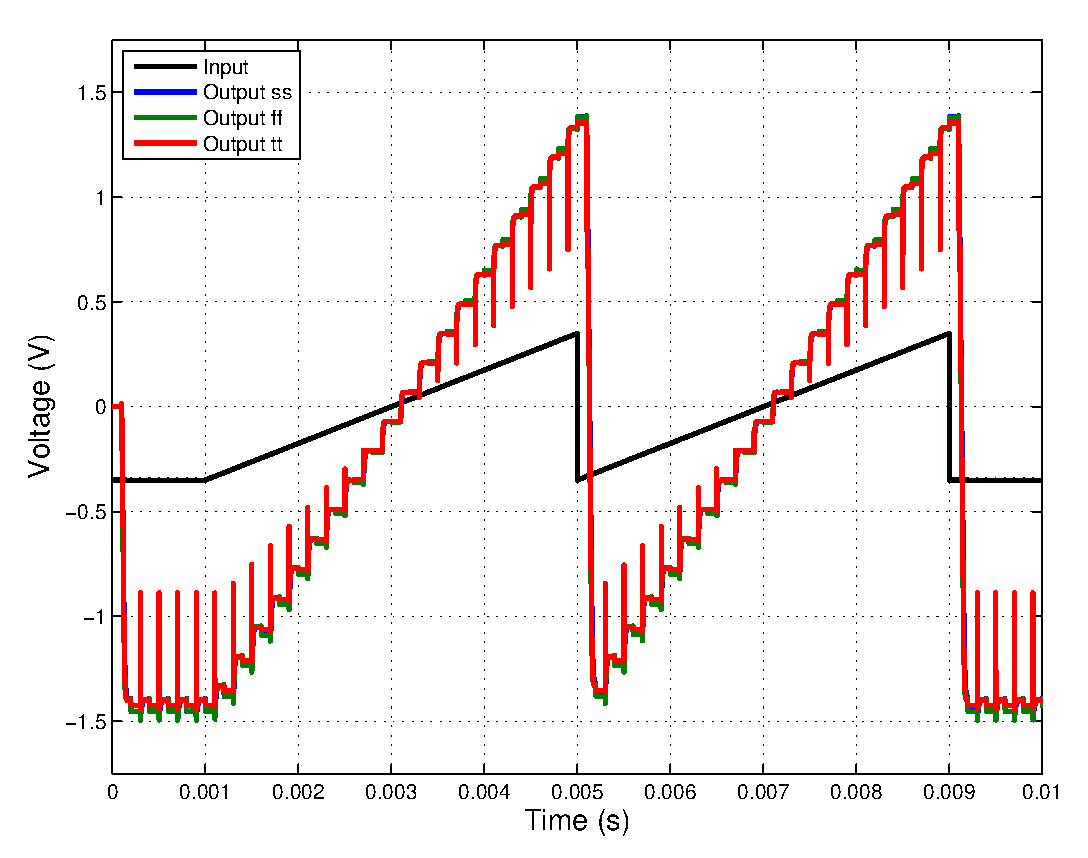
\includegraphics[width=4in]{Plots/closed_saw.eps}
\caption{The closed loop transient response to a full-scale amplitude sawtooth with a frequency of $\frac{f_s}{20}$.}
\label{fig:closed_saw}
\end{figure}

\subsection{Effective Number of Bits}

\subsection{Figure of Merit}
We calculated our figure of merit based on both the DC power consumption of our system as well as the average overall power of our system. Both values of power are shown in table \ref{tab:specs_results} and the FOM values are shown below.

\begin{equation}
FOM_{DC-POWER} = \frac{Power_{dc}}{2^{ENOB}f_s} = 150.3 fJ
\end{equation}

\begin{equation}
FOM_{TOTAL-POWER} = \frac{Power_{total}}{2^{ENOB}f_s} = 441.4 fJ
\end{equation}

\subsection{Area}
With the functionality of our system verified and its performance measured, we made an estimation of the area of our design. To measure the area of the transistors in the design, we used the below formula where $L_{diff} = 0.48 \mu m$ and $\alpha = 1.3$.

\begin{equation}
Area_{transistors} = W*(L+L_{diff})*\alpha = 55.50 pm^2
\end{equation}

To calculate the area of the capacitors in our circuit, we used the below formula across all of our capacitors where $C_{unit-area} = 1fF/\mu m^2$.

\begin{equation}
Area_{capacitors} = \sum{C/C_{unit-area}} = 3.00 nm^2
\end{equation}

Finally, to calculate the area of the resistors in our circuit, we used the below formula across all of the resistors in our design where $R_s = 10\Omega / \mu m^2$.

\begin{equation}
Area_{resistors} = \sum{R/R_s} = 8.00 \mu m^2
\end{equation}

Adding the above results for area, we came to a total area estimation as shown below.

\begin{equation}
Area_{total} = 8.0036 \mu m^2
\end{equation}

\section{Summary of Results}
As can be gathered from our numerical results, we successfully reached the goal we set out to accomplish. We designed a $10bit$, $5k sample/s$ amplifier for use in a $2.5bit/stage$ pipelined analog-to-digital converter which settles to an input referred error value less than $\frac{V_{LSB}}{2}$. In the process of designing this amplifier, we were able to maintain a very low value of total power consumption and as a result, a very respectable figure of merit. Thanks to a well thought out design process, we built and amplifier that not only meets its specs, but also maintains those specs over all PVT corners. If this design was put onto silicon and distributed to customers, we believe that it would prove to be robust enough to handle constant unpredictable use.

\begin{table}
\centering
\caption{Summary of Specifications and Results}
\label{tab:specs_results}
\begin{tabular}{|c|c|c|c|c|}
\hline Specification & Specification Value & FF Result & TT Result & SS Result\\ 
\hline Open Loop OTA DC Gain & $72.20 dB$ &$102.38 dB$&$110.86 dB$&$112.57 dB$\\ 
\hline Open Loop OTA Phase Margin & $60^o$ & $75.4^o$ & $75.2^o$ & $74.3^o$ \\ 
\hline Open Loop OTA Unity Gain Bandwidth & $44.10kHz$ & $96.93kHz$ & $87.34 kHz$ &  $68.83 kHz$ \\ 
\hline DC Power Consumption & -- & $747.90 nW$ & $769.50 nW$ & $803.16 nW$\\ 
\hline Overall Power Consumption & -- & -- & $2.26\mu W$ & --\\ 
\hline DC Figure of Merit & -- & -- & $150.3 fJ$ & --\\ 
\hline Overall Figure of Merit & -- & -- & $441.4 fJ$ & --\\ 
\hline Overall Area & -- & -- & $8.0036 \mu m^2$ & -- \\ 
\hline 
\end{tabular} 
\end{table}


\section{Possible Improvements}
While most of the specifications of our finished amplifier are impressive, one that needs optimization is the total area. Because we originally set out to meet a more stringent specification for gain, we were forced to utilize two $40\Omega$ resistors in the CMFB circuit. These two resistors account for the vast majority of the design's area. Because we ultimately were able to attain a gain far greater than the requirement, in future optimizations of the design we would focus on bringing the value (and hence size) of these resistors down to a more reasonable value. In addition, we believe that with redesign of the OTA, we can achieve a much lower power consumption and utilize much smaller compensation capacitors.

\section{Conclusion}
Through the design of this amplifier, we were able to attain a good deal of knowledge on new circuit techniques as well as design process. Unlike some of our previous designs, we spent a very long time developing our ideas on paper until we were satisfied that they would give us the results we were looking for. Thanks to this patience, once we put our theories into simulation, we were very pleased with the results. We were able to hit our spec after the first iteration of design and we spent most of the remaining design time optimizing for power and accuracy.
This project is quite appropriate for the class because it allows a broad range of students with different backgrounds to show interest. Because the design requires some knowledge of digital theory in addition to the heavy analog theory, a strong need for collaboration was instilled and led to a much more organic learning environment. 

% references section

% can use a bibliography generated by BibTeX as a .bbl file
% BibTeX documentation can be easily obtained at:
% http://www.ctan.org/tex-archive/biblio/bibtex/contrib/doc/
% The IEEEtran BibTeX style support page is at:
% http://www.michaelshell.org/tex/ieeetran/bibtex/
%\bibliographystyle{IEEEtran}
% argument is your BibTeX string definitions and bibliography database(s)
%\bibliography{IEEEabrv,../bib/paper}
%
% <OR> manually copy in the resultant .bbl file
% set second argument of \begin to the number of references
% (used to reserve space for the reference number labels box)
%%\begin{thebibliography}{1}
%%
%%\bibitem{sedrasmith}
%%A.~Sedra and K.~Smith, \emph{Microelectronic Circuits}, 6th~ed. \\ 
%%Oxford University Group, 2009. pgs. 711-716.  
%%\bibitem{LowGroupDelay}
%%Kim, J.; Buckwalter, J.F.; "Bandwidth Enhancement With Low Group-Delay Variation for a 40-Gb/s Transimpedance Amplifier," \emph{Circuits and Systems I: Regular Papers, IEEE Transactions on} , vol.57, no.8, pp.1964-1972, Aug. 2010.
%%
%%\end{thebibliography}

%\bibliographystyle{plain}
%\bibliography{AnalogProjectReferences}

\section{Seminar Responses: Miles Sherman}
\subsection{Simone Gambini: More Than Moore Systems}
Dr. Gambini gave an informative and interesting perspective on his work and the industry as a whole. While I was previously aware of a good amount of "More Than Moore" work being done, getting a feel for some specific projects was helpful for my understanding. The one aspect of this seminar that stuck with me was the fact that the noise associated with actually stimulating brain activity is actually larger than the brain's signal poses an interesting problem and a demand for a solution. There is definitely a lot of room for major development in this field.

\subsection{Adad Abidi: Armstrong's Circuits \& The Worldwide Spread of Radio}
Of the three seminars I attended this semester, I would say this one was the most interesting for me. Dr. Abidi presented the work of Edwin Armstrong in a very specific way so as to motivate a connection between the work of the 1920's and the analog design of today. Armstrong's circuits played a major role in influencing the way we communicate today and it is	clear when his fundamental designs are found in the large systems of analog communication chips in modern day devices. Armstrong's main focus in his work seems to be resourcefulness since vacuum tubes were so expensive. Modern day engineers can learn a lot from his work. Even though transistors are a commodity now, there is always optimization to be done.

\subsection{Shanthi Pavan: Continuous-Time Delta Sigma Data Converters}
This was the final lecture I attended and I probably had the most trouble following this one due to its more in depth technical discussion of a new topic for me. Dr. Pavan discussed new techniques for the elimination of clock-jitter and non-linearities in delta sigma converters. While I could not follow his exact method of innovation, I was certainly able to learn a good amount about the operation of delta sigma converters. These systems operate by oversampling the input at sampling rates much higher than those at the final output of the system. By doing this, the system can then modulate the noise and push it to higher frequencies than those of interest. The signal is then re-sampled and outputted.

\end{document}